En el capítulo anterior vimos que, a temperaturas suficientemente bajas o densidades altas, la aproximación clásica dejaba de ser válida para el estudio de las propiedades termodinámicas de los gases.
La experiencia confirma esta predicción teórica, y así se observa, por ejemplo, en el caso de hidrógeno y del helio, que a bajas temperaturas las discrepancias entre los resultados experimentales y los predichos por la teoría clásica se vuelven muy importantes.
Hay que señalar que esta discrepancia no es meramente cuantitativa, sino que se presentan efectos que requieren una descripción mecánico-cuántica del modelo considerado para su simple explicación cualitativa.

En este capítulo vamos a estudiar algunos de estos efectos en el caso de gases ideales.
Es decir, de acuerdo con la nomenclatura introducida en el capítulo anterior, vamos a estudiar gases ideales fuertemente degenerados. Como veremos, los desarrollos y las propiedades que se obtienen son muy distintas en el caso de fermiones y en el caso de bosones, por lo que estudiaremos ambos por separado.

\newpage
\section{Gas de Fermi-Dirac. Cálculo de valores medios a T=0K.}

El número de fermiones en un estado de partícula $r$ viene dado de acuerdo con \eqref{eq:n_r_1} por
\begin{equation}\label{eq:n_r_t8}
	\expval{n_r} = \frac{1}{e^{\beta\varepsilon_r + \alpha} + 1}
\end{equation}

Sabemos, además, que el número de estados de traslación de una partícula en el intervalo de energía comprendido entre $\varepsilon$ y $\varepsilon+d\varepsilon$ viene dado por \eqref{eq:D_vareps}.
Este número no coincide, sin embargo, con el número de estados de un electrón en el intervalo de energía considerado, En efecto, la especificación del estado de un electrón ---y de toda partícula con espín--- exige conocer también su estado de espín, o sea la orientación del mismo.
En el caso de electrones, que tienen espín $\sfrac{1}{2}$, son posibles dos orientaciones o rotados de espín.
Como estamos considerando un sistema aislado, la energía de un electrón será independiente de la orientación de su espín, resultando que con cada estado de traslación son posibles dos estados de espín que corresponden a la misma energía.\footnote{Evidentemente, como ocurre para el momento cinético ordinario, para partículas que no tengan espín $\sfrac{1}{2}$, el número de estados de espín por cada estado de traslación no será 2, sino en general $2s + 1$, siendo $s$ el valor del número cuántico de espín.}

En resumen, el número de estados electrónicos con energía comprendida entre $\varepsilon$ y $\varepsilon+d\varepsilon$ será
\begin{equation}
	D(\varepsilon) d\varepsilon = 2\frac{4\pi V}{h^3} (2m^3)^{1/2} \varepsilon^{1/2} d\varepsilon
\end{equation}

Conocido el número de estados y el número medio de electrones en cada estado ---que depende solo de la energía del mismo---, podemos calcular la siguiente función:
\begin{equation}
	f(\varepsilon) d\varepsilon \equiv \parbox{28em}{número medio de electrones que en el sistema de volumen $V$ \\tiene una energía comprendida entre $\varepsilon$ y $\varepsilon+d\varepsilon$} 
\end{equation}
y que vendrá dada por
\begin{equation}\label{eq:f_e}
	f(\varepsilon) d\varepsilon = D(\varepsilon)\expval{n_r} d\varepsilon = \frac{8\pi V}{h^3} (2m^3)^{1/2} \frac{\varepsilon^{1/2}}{e^{\beta(\varepsilon_r -\mu)} + 1} \dd{\varepsilon}
\end{equation}

\begin{wrapfigure}{r}{0.35\textwidth}
	\centering
	\hspace{1.8cm}
	% This file was created by matplotlib2tikz v0.6.16.
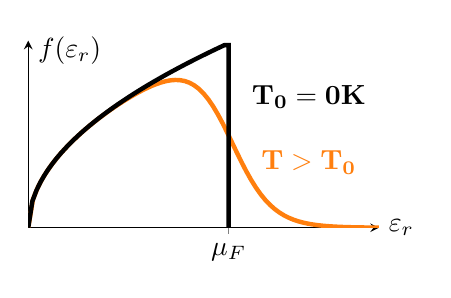
\begin{tikzpicture}

\definecolor{color0}{rgb}{0.12156862745098,0.466666666666667,0.705882352941177}
\definecolor{color1}{rgb}{1,0.498039215686275,0.0549019607843137}

\begin{axis}[
scale = 0.65,
axis lines = left,
y = 0.85cm,
xmin=0, xmax=3.5,
ymin=0, ymax=4.3,
every axis x label/.style={at={(current axis.right of origin)},anchor=west},
ylabel style={at={(ticklabel* cs:0.82)},anchor=south west, rotate=-90},
ytick=\empty,
xtick={2},
xlabel = {$\varepsilon_r$},
ylabel = {$f(\varepsilon_r)$},
xticklabel = {$\mu_F$},
tick pos=left]

\node at (2.8,3) {$\mathbf{T_0 = 0K}$};
\node at (2.8,1.5) {$\color{color1}\mathbf{T > T_0}$};

\addplot [ultra thick, color1, forget plot]
table {%
0 0
0.0472972972972973 0.652400733301861
0.0945945945945946 0.922619809546396
0.141891891891892 1.12995191841971
0.189189189189189 1.30472396537706
0.236486486486487 1.45868024525444
0.283783783783784 1.59784102152928
0.331081081081081 1.72577918731048
0.378378378378378 1.84481860301694
0.425675675675676 1.9565684976473
0.472972972972973 2.06219451885098
0.52027027027027 2.16256922445519
0.567567567567568 2.25836133076218
0.614864864864865 2.35009122818548
0.662162162162162 2.43816662422642
0.70945945945946 2.5229057473735
0.756756756756757 2.60455228276139
0.804054054054054 2.68328444224755
0.851351351351351 2.75921955382751
0.898648648648649 2.83241493369093
0.945945945945946 2.90286540122466
0.993243243243243 2.97049752156059
1.04054054054054 3.03516046634594
1.08783783783784 3.09661325375866
1.13513513513514 3.15450806704296
1.18243243243243 3.20836938115471
1.22972972972973 3.25756879734636
1.27702702702703 3.30129587261222
1.32432432432432 3.33852594586442
1.37162162162162 3.36798715026668
1.41891891891892 3.38813062437796
1.46621621621622 3.39711052766342
1.51351351351351 3.39278382956826
1.56081081081081 3.37274365693506
1.60810810810811 3.3344033373232
1.65540540540541 3.27514935295824
1.7027027027027 3.19257739249026
1.75 3.08481319018989
1.7972972972973 2.95089657368637
1.84459459459459 2.79117475351894
1.89189189189189 2.60761811079186
1.93918918918919 2.4039548607329
1.98648648648649 2.18553811514009
2.03378378378378 1.95891779705724
2.08108108108108 1.7311763224055
2.12837837837838 1.50916547689593
2.17567567567568 1.29881427254418
2.22297297297297 1.1046477847626
2.27027027027027 0.929582110861403
2.31756756756757 0.774978038345978
2.36486486486486 0.640879018982362
2.41216216216216 0.526340409645743
2.45945945945946 0.429769501401771
2.50675675675676 0.34922349151626
2.55405405405405 0.282640877603157
2.60135135135135 0.228002913077345
2.64864864864865 0.183433958782042
2.69594594594595 0.147254435096629
2.74324324324324 0.11800029418219
2.79054054054054 0.0944208424913346
2.83783783783784 0.0754639281856427
2.88513513513514 0.0602548258556417
2.93243243243243 0.0480729598526281
2.97972972972973 0.0383289785586019
3.02702702702703 0.0305435615491269
3.07432432432432 0.0243286018854659
3.12162162162162 0.0193709491384576
3.16891891891892 0.0154186358196685
3.21621621621622 0.0122693732894764
3.26351351351351 0.00976104523843906
3.31081081081081 0.00776391530132588
3.35810810810811 0.00617427936728086
3.40540540540541 0.00490931963432403
3.4527027027027 0.00390294858807993
3.5 0.00310246240514403
};
\addplot [ultra thick, black, forget plot]
table {%
0 0
0.0408163265306122 0.606091526731326
0.0816326530612245 0.857142857142857
0.122448979591837 1.04978131833565
0.163265306122449 1.21218305346265
0.204081632653061 1.35526185435788
0.244897959183673 1.48461497791618
0.285714285714286 1.60356745147455
0.326530612244898 1.71428571428571
0.36734693877551 1.81827458019398
0.408163265306122 1.91662969499982
0.448979591836735 2.01017818278147
0.489795918367347 2.0995626366713
0.530612244897959 2.18529407725405
0.571428571428571 2.26778683805536
0.612244897959184 2.34738238930785
0.653061224489796 2.42436610692531
0.693877551020408 2.49897938350513
0.73469387755102 2.57142857142857
0.775510204081633 2.64189171555813
0.816326530612245 2.71052370871575
0.857142857142857 2.77746029931765
0.897959183673469 2.84282124887606
0.938775510204082 2.90671284991083
0.979591836734694 2.96922995583236
1.02040816326531 3.03045763365663
1.06122448979592 3.09047252182628
1.10204081632653 3.14934395500694
1.14285714285714 3.20713490294909
1.18367346938776 3.26390275965596
1.22448979591837 3.31970001103493
1.26530612244898 3.37457480314792
1.30612244897959 3.42857142857143
1.3469387755102 3.48173074484398
1.38775510204082 3.53409053624371
1.42857142857143 3.58568582800318
1.46938775510204 3.63654916038796
1.51020408163265 3.68671082873255
1.55102040816327 3.73619909446343
1.59183673469388 3.78504037128336
1.63265306122449 3.83325938999964
1.6734693877551 3.88087934491604
1.71428571428571 3.92792202424786
1.75510204081633 3.97440792664102
1.79591836734694 4.02035636556294
1.83673469387755 4.06578556307363
1.87755102040816 4.11071273426804
1.91836734693878 4.15515416349971
1.95918367346939 4.19912527334259
2 4.2
2.00001 0
};
\end{axis}

\end{tikzpicture}
	\vspace{-1cm}
\end{wrapfigure}
Notemos que para escribir esta expresión, hemos considerado a $\varepsilon_r$ en \eqref{eq:n_r_t8} como un parámetro continuo.
La justificación para ello es la proximidad de los niveles energéticos, que fue de hecho lo que nos permitió también definir una densidad de estados por unidad de intervalo de energía.

A partir de \eqref{eq:f_e} podemos escribir para el número de electrones que constituyen el sistema y para la energía media del gas las expresiones
\begin{align}
	N &= \int_{0}^{\infty} \dd{\varepsilon} f(\varepsilon) = \frac{8\pi V}{h^3} (2m^3)^{1/2} \int_{0}^{\infty} \dd{\varepsilon} \frac{\varepsilon^{1/2}}{e^{\beta\varepsilon_r + \alpha} + 1} \label{eq:N_FD}\\
	\expval{E} &= \int_{0}^{\infty} \dd{\varepsilon} \varepsilon f(\varepsilon) = \frac{8\pi V}{h^3} (2m^3)^{1/2} \int_{0}^{\infty} \dd{\varepsilon} \frac{\varepsilon^{3/2}}{e^{\beta\varepsilon_r + \alpha} + 1}
\end{align}

Nosotros consideraremos siempre un sistema cerrado, de manera que la primera de estas ecuaciones es precisamente la que define el valor del nivel de Fermi $\mu_F$.

Si particularizamos estas dos ecuaciones para $T = 0 K$ resulta, en virtud de lo que acabamos de decir
\begin{align}
	N &=  \frac{8\pi V}{h^3} (2m^3)^{1/2} \int_{0}^{\mu_F} \dd{\varepsilon} \varepsilon^{1/2} = \frac{16\pi V}{3h^3} (2m^3)^{1/2} \mu_F^{3/2}\\
	\expval{E} &=  \frac{8\pi V}{h^3} (2m^3)^{1/2} \int_{0}^{\mu_F} \dd{\varepsilon} \varepsilon^{3/2} = \frac{16\pi V}{5h^3} (2m^3)^{1/2} \mu_F^{5/2}
\end{align}

De la primera de estas ecuaciones se obtiene para la energía de Fermi
\begin{equation}
	\mu_F = \frac{h^2}{8m} \left( \frac{3N}{\pi V}\right)^{3/2}
\end{equation}
mientras que de la comparación de ambas resulta
\begin{equation}
	\expval{E} = \frac{3}{5} N \mu_F
\end{equation}

\textit{[TBC]}

\section{Propiedades termodinámicas}

\section{Gas de Fermi-Dirac para T<0K. Cálculo de valores medios}

\section{Gas de Bose-Einstein degenerado. Condensación de Bose-Einstein}

Pasemos a considerar un gas ideal de bosones degenerado.
Como ya dijimos al principio de este capítulo, el comportamiento, en condiciones de degeneración, de un gas de Bose es muy distinto al de un gas de Fermi.
Esta diferencia es previsible, pues en un gas de Bose, al disminuir la temperatura, las partículas pueden agruparse en los estados de menor energía, mientras que en un gas de Fermi existen, incluso en el límite $T \rightarrow 0$, partículas en niveles relativamente altos de energía, debido al principio de exclusión de Pauli.
Más concretamente, sabemos que en el cero absoluto el límite superior de energías es la energía de Fermi.

El número medio de partículas en un estado cuántico $r$ es en el caso de bosones
\begin{equation}\label{eq:n_r_BE}
	\expval{n_r} = \frac{1}{e^{\beta(\varepsilon_r -\mu)} - 1}
\end{equation}
y, por lo tanto, si el sistema contiene N partículas debe cumplirse
\begin{equation}\label{eq:N_BE}
	N = \sum_r \frac{1}{e^{\beta(\varepsilon_r -\mu)} - 1}
\end{equation}

Recordemos que por considerar un sistema cerrado esta ecuación es precisamente la que nos determina el potencial químico $\mu$.

Supongamos ahora que el nivel más bajo de energía accesible a una partícula es $\varepsilon = 0$.\footnote{Esto no es una hipótesis, sino que coincide con nuestros resultados. En efecto, la energía asociada con el movimiento de traslación es la única energía que poseen las partículas de un gas ideal aislado. Cuando consideramos un sistema suficientemente grande es claro que el nivel más bajo de energía tiende a cero.}
A partir de \eqref{eq:n_r_BE} obtenemos que
\begin{equation}\label{eq:mu_t_BE}
	\mu(T) \leq 0
\end{equation}
ya que en otro caso existirán estados ---en particular el o los correspondientes a $\varepsilon_r = 0$--- para los que $\varepsilon_r -\mu < 0$ y $\exp[\beta(\varepsilon_r -\mu)] < 1$, de manera que resultaría $\expval{n_r} < 0$, que no tiene sentido.
De hecho, para obtener \eqref{eq:n_r_BE} nos fue necesario admitir que se cumplía \eqref{eq:cond_FD}, que se convierte en \eqref{eq:mu_t_BE}, al considerar que el valor mínimo de $\varepsilon_r$ es cero.

Vamos a tratar de estudiar el gas de Bose degenerado de manera análoga a como hemos realizado el análisis del gas de Fermi.
Para ello consideremos la expresión que se obtiene al explicitar en \eqref{eq:N_BE} la suma respecto de los estados de traslación, o sea la expresión análoga a \eqref{eq:N_FD}
\begin{align}\label{eq:N_2_BE}
	N &= \int_0^{\infty} \dd{\varepsilon} f(\varepsilon) = \int_0^{\infty} \dd{\varepsilon} D(\varepsilon) \expval{n_r}(\varepsilon) \nonumber \\
	&= g \frac{4\pi V}{h^3} (2m^3)^{1/2} \int_0^{\infty} \dd{\varepsilon} \frac{\varepsilon^{1/2}}{e^{\beta(\varepsilon -\mu)} - 1}
\end{align}

Las diferencias existentes respecto a \eqref{eq:N_FD} son dos: la sustitución de la distribución de Fermi por la de Bose y del factor 2 asociado a los electrones, para los que $s = 1/2$, por un factor de degeneración más genérico $g = 2s + 1$.

Si para una densidad dada del gas, $\sfrac{N}{V}$, disminuimos la temperatura ---aumentamos $\beta$--- las diferencias $\varepsilon -\mu$ tendrán que disminuir para que la integral que aparece en \eqref{eq:N_2_BE} puede conservar su valor.
Como $\varepsilon -\mu = \abs{\varepsilon} + \abs{\mu}$, resulta que, al disminuir la temperatura disminuye en valor absoluto $\mu$, que es negativo.
Como acabamos de ver que $\mu$ no puede ser positivo, resultará que $\mu$ irá aumentando hasta alcanzar el valor límite $\mu = 0$. La temperatura $T_0$ a la cual se alcanza este valor vendrá definida por la igualdad $\beta_0 = 1/k_BT_0$
\begin{align}
	N &= g \frac{4\pi V}{h^3} (2m^3)^{1/2} \int_0^{\infty} \frac{\varepsilon^{1/2}}{e^{\beta_0\varepsilon } - 1} \nonumber \\
	&= g \frac{4\pi V}{h^3} (2m^3)^{1/2} \beta_0^{-3/2} \int_0^{\infty} \dd{z} \frac{z^{1/2}}{e^z - 1}
\end{align}
donde hemos efectuado el cambio de variable $z = \varepsilon\beta_0$.
La integral que aparece en esta está resulta en el \hyperref[Anx5]{Anexo 5}, que nos permite escribir la anterior ecuación en la forma
\begin{equation}\label{eq:N/V_BE}
	\frac{N}{V} = \frac{2\pi \sqrt{\pi}}{h^3} (2m^3)^{1/2} \zeta(\sfrac{3}{2}) \beta_0^{-3/2}
\end{equation}
de donde se obtiene
\begin{equation}\label{eq:T_0_BE}
	T_0 = \frac{h^2}{2\pi mk_B} \left[ \frac{N}{gV\zeta(\sfrac{3}{2})} \right]^{2/3} = 3,31 \frac{\hbar^2}{km^{5/3}} \left[ \frac{Nm}{g} \right]^{2/3} 
\end{equation}

Resulta entonces que para temperaturas inferiores a $T_0$ la expresión \eqref{eq:N_2_BE} no tiene sentido, pues es imposible encontrar un valor de $\mu$ que la satisfaga ---evidentemente, para $\mu > 0$ la integral es divergente, pues el denominador tiende a cero cuando $\varepsilon$ tiende a $\mu$---.

Veamos otro modo de interpretar los resultados obtenidos.
Podemos imaginar ahora que mantenemos constante la temperatura, aumentando el número de partículas del sistema.
De acuerdo con \eqref{eq:N_2_BE}, aumento de $N$ exigirá una disminución de $\exp[\beta(\varepsilon_r -\mu)]$ y, por lo tanto, un aumento de $\mu$ que es negativo como sabemos.
¿Hasta qué valor podemos aumentar $N$ de modo que se satisfaga \eqref{eq:N_2_BE}? Pues hasta alcanzar el valor límite $\mu = 0$.
Es decir, que el valor del número máximo de partículas que según \eqref{eq:N_2_BE} podría tener el sistema a una temperatura $T$ vendría dado por
\begin{equation}\label{eq:N/V_max_BE}
	\frac{N_{max}}{V} = \frac{2\pi \sqrt{\pi}}{h^3} (2m^3)^{1/2} \zeta(\sfrac{3}{2}) \beta^{-3/2}
\end{equation}

Resultaría, según esto, que en un gas de bosones el número de partículas estaría acotado y, además, sería proporcional a $T^{3/2}$, lo que en particular implicaría que no podría existir un gas de bosones en el límite $T \rightarrow 0$.
Tratemos de entender lo que ha sucedido y volvamos a \eqref{eq:n_r_BE} y \eqref{eq:N_BE}, haciendo tender $T$ a cero. Es evidente que
$$\expval{n_r}(\varepsilon_r - \mu) \rightarrow 0$$
y
$$N = g\expval{n_r} = g \frac{1}{e^{-\beta\mu} - 1}$$

En esta última ecuación siempre podría ajustarse $\mu$ de manera que se cumpliese la igualdad por pequeña que fuese $T$ ---$\beta$ grande---.
En particular, mientras no sea $T$ idénticamente cero es evidente que $\mu \rightarrow 0$ lleva a $N \rightarrow \infty$.

Resulta entonces que la.s dificultades han aparecido al pasar de \eqref{eq:N_BE} a \eqref{eq:N_2_BE}, es decir, al introducir la densidad de estados $D(\varepsilon)$ que es todo lo que necesitamos para pasar de una a otra.
En este paso se ha utilizado el valor
\begin{equation}\label{eq:D_vareps_BE}
	D(\varepsilon) dd{\varepsilon} = g \frac{4\pi V\sqrt{2m^3}}{h^3} (2m^3)^{1/2} \varepsilon^{1/2} dd{\varepsilon}
\end{equation}
que se obtiene al sustituir los niveles discretos de energía por una distribución continua sobre toda la recta real.
Si en esta ecuación tomamos el límite $\varepsilon \rightarrow 0$, Y debido al factor $\varepsilon^{1/2}$, obtenemos
$$\lim\limits_{\varepsilon \rightarrow 0} D(\varepsilon) = 0$$
y análogamente en el caso del número de partículas por unidad de intervalo de energía:
$$\lim\limits_{\varepsilon \rightarrow 0} f(\varepsilon) = 0$$

Así, pues, al admitir el paso a un espectro continuo en el sentido considerado hasta ahora, estamos implícitamente admitiendo que el número medio de partículas en el estado ---o los estados--- de energía $\varepsilon \rightarrow 0$ es nulo.
Este hecho no tiene importancia en la estadística de Fermi, donde en cada estado puede haber como máximo una partícula, ni en la estadística de Bose a temperaturas altas, en que el número de partículas en $\varepsilon \rightarrow 0$ es muchísimo menor que el número total de partículas que contiene el sistema.
Sin embargo, en el caso de un gas de Bose a temperaturas suficientemente bajas, la existencia de un estado de traslación que corresponde a $\varepsilon = 0$ es de fundamental importancia puesto que, como hemos visto antes, las partículas tienden a agruparse precisamente en ese nivel energético.

Para solucionar esta dificultad hemos de escribir el sumatorio \eqref{eq:N_BE} en la forma
\begin{equation}\label{eq:N_3_BE}
	N = g \frac{1}{e^{-\beta\mu} - 1} + \sum_{\substack{r\\(\varepsilon_r \neq 0)}} \frac{1}{e^{\beta(\varepsilon_r -\mu)} - 1}
\end{equation}

El segundo sumando del esta expresión es el que puede aproximarse por una integral, de manera que en lugar de \eqref{eq:N_2_BE} la expresión correcta será
\begin{equation}\label{eq:N_4_BE}
	N = N_0 + N' 
\end{equation}
donde $N_0$ representa el número de partículas en el nivel fundamental $(\varepsilon = 0)$ y $N'$ el número de partículas en estados excitados ---$\varepsilon > 0$---. Es decir,
\begin{equation}
	N_0 = g \frac{1}{e^{-\beta\mu} - 1}
\end{equation}
\begin{equation}
	N' = g \frac{4\pi V\sqrt{2m^3}}{h^3} (2m^3)^{1/2} \int_{0}^{\infty} \frac{\varepsilon^{1/2}}{e^{\beta(\varepsilon -\mu)} - 1}
\end{equation}

El estudio de las propiedades de un gas de Bose degenerado sobre todo el rango de temperaturas es muy complicado y requiere el empleo del cálculo numérico, por lo que nos vamos a limitar aquí a una discursión cualitativa.

a) Consideremos el gas de Bose a una cierta densidad $\sfrac{N}{V}$ y a una temperatura $T \gg T_0$, siendo $T_0$ la temperatura definida por \eqref{eq:T_0_BE}.
A partir de \eqref{eq:N/V_BE} y \eqref{eq:N/V_max_BE} obtenemos que
\begin{equation}\label{eq:N/N_max}
	\frac{N_{max}}{N} = \left( \frac{T}{T_0} \right)^{3/2}
\end{equation}
que en la zona que estamos considerando es mucho mayor que la unidad.
Es decir, que para $T \gg T_0$ el número máximo de partículas que pueden existir en estados excitados es mucho mayor, que $N$.
Resulta entonces que prácticamente todas las partículas se encuentran en estados excitados, lo que corresponde a $\abs{\mu} \gg T_0$ y
\begin{equation}
	N_0 = g \frac{1}{e^{-\beta\mu} - 1} \ll 1
\end{equation}

b) Disminuyamos ahora la temperatura, manteniendo $\sfrac{N}{V}$ constante.
Al alcanzar $T = T_0$ se hace $N = N'_{max}$.
Hay que observar ahora claramente que $N = N'_{max}$ no implica que $\mu$ sea nulo.
Ambas cosas eran equivalentes cuando no considerábamos ---erróneamente--- el estado fundamental, pero una vez introducida la descomposición \eqref{eq:N_4_BE}, aunque sea $N = N'_{max}$ el potencial químico será todavía distinto a cero ---aunque muy pequeño--- y el número de partículas en estados excitados será menor que $N'_{max}$

c) Si seguimos disminuyendo la temperatura por trabajo de $T_0$, $N'_{max}$ continuará disminuyendo y en consecuencia el número de partículas en el estado fundamental irá aumentando.
Para temperaturas menores que $T_0$ puede escribirse
\begin{equation}
	N_0 = N - N' \simeq N - N'_{max}
\end{equation}
o utilizando \eqref{eq:N/N_max}
\begin{equation}
	N_0 = N  \left[ 1 - \left( \frac{T}{T_0} \right)^{3/2} \right]
\end{equation}

\begin{wrapfigure}[6]{l}{0.4\textwidth}
	\centering
	% This file was created by matplotlib2tikz v0.6.16.
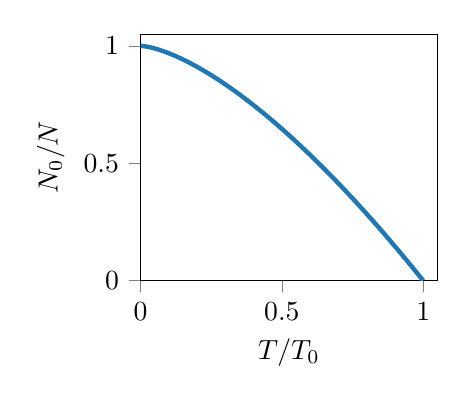
\begin{tikzpicture}

\definecolor{color0}{rgb}{0.12156862745098,0.466666666666667,0.705882352941177}

\begin{axis}[
scale = 0.55,
xmin=0, xmax=1.05,
ymin=0, ymax=1.05,
tick align=outside,
tick pos=left,
ylabel = {$N_0/N$},
xlabel = {$T/T_0$},
x grid style={white!69.01960784313725!black},
y grid style={white!69.01960784313725!black}
]
\addplot [ultra thick, color0, forget plot]
table {%
0 1
0.0204081632653061 0.997084548104956
0.0408163265306122 0.991753856779166
0.0612244897959184 0.984850867572284
0.0816326530612245 0.97667638483965
0.102040816326531 0.967404256887758
0.122448979591837 0.957151782925076
0.142857142857143 0.946005075284396
0.163265306122449 0.934030854233325
0.183673469387755 0.921282798833819
0.204081632653061 0.907805316030076
0.224489795918367 0.893635939667903
0.244897959183673 0.878806940578271
0.26530612244898 0.863346453116525
0.285714285714286 0.847279290335758
0.306122448979592 0.830627550457402
0.326530612244898 0.813411078717201
0.346938775510204 0.795647826135568
0.36734693877551 0.777354133037472
0.387755102040816 0.758544956480254
0.408163265306122 0.739234055102065
0.428571428571429 0.719434141125153
0.448979591836735 0.699157006658556
0.469387755102041 0.678413629632092
0.489795918367347 0.657214263400605
0.510204081632653 0.635568513119533
0.530612244897959 0.613485401302005
0.551020408163265 0.590973424451665
0.571428571428571 0.568040602275169
0.591836734693878 0.54469452067959
0.612244897959184 0.520942369529009
0.63265306122449 0.496790975954138
0.653061224489796 0.4722468338666
0.673469387755102 0.447316130216458
0.693877551020408 0.422004768440991
0.714285714285714 0.396318389479631
0.73469387755102 0.370262390670554
0.755102040816326 0.343841942795819
0.775510204081633 0.317062005501979
0.795918367346939 0.289927341289978
0.816326530612245 0.262442528240611
0.836734693877551 0.234611971618814
0.857142857142857 0.20643991448067
0.877551020408163 0.177930447390711
0.897959183673469 0.149087517343221
0.918367346938775 0.119914935969471
0.938775510204082 0.0904163871027338
0.959183673469388 0.0605954337642884
0.979591836734694 0.0304555246261679
1 0
};
\end{axis}

\end{tikzpicture}
	\vspace{-0.65cm}
\end{wrapfigure}

Además, a estas temperaturas el potencial químico $\mu$ es ya prácticamente nulo.
Cuando más se disminuye la temperatura más y más partículas se agrupan en el nivel fundamental ---$\varepsilon = 0$---.
En la figura se representa el comportamiento de $\sfrac{N_0}{N}$ frente a $\sfrac{T}{T_0}$.

\newpage
Este fenómeno recibe el nombre de \emph{condensación de Bose-Einstein}, denominándose a $T_0$ \emph{temperatura de condensación}, ya que en cierto sentido recuerda el proceso de condensación de un vapor en la fase líquida.
Sin embargo, estos dos procesos son conceptualmente muy diferentes.
En la condensación normal de un gas, las partículas se agrupan en un cierto volumen que depende de la densidad del líquido y de la cantidad de gas condensado, lo que se traduce en una acumulación de puntos representativos en el espacio de las fases en una zona correspondiente a un intervalo limitado de posiciones.
Por el contrario, en la condensación de Base-Einstein, la agrupación tiene lugar en el espacio de momentos, concretamente alrededor del valor $p = 0$.

\section{Propiedades del gas de Bose para T<T\textsubscript{0}}

Para temperaturas inferiores a $T_0$ sabemos que $\mu$ es muy pequeño de forma que puede escribirse con buena aproximación
\begin{equation}
	\expval{E} = g \frac{4\pi V}{h^3} (2m^3)^{1/2} \int_0^{\infty} \dd{\varepsilon} \frac{\varepsilon^{1/2}}{e^{ \beta\epsilon} - 1}
\end{equation}
donde hemos tenido en cuenta que las $N_0$ partículas existentes en el estado fundamental poseen una energía nula.
Haciendo el cambio de variable $z = \beta\varepsilon$ obtenemos
\begin{equation}
	\expval{E} = g \frac{4\pi V}{h^3} (2m^3)^{1/2} \beta^{-5/2} \int_0^{\infty} \dd{z} \frac{z^{3/2}}{e^z - 1}
\end{equation}
que podemos resolver con el \hyperref[Anx5]{Anexo 5}
\begin{equation}
	\expval{E} = g \frac{4\pi V}{h^3} (2m^3)^{1/2} \, \beta^{-5/2} \, \Gamma\left( \sfrac{5}{2} \right) \zeta\left( \sfrac{5}{2} \right) 
\end{equation}

Si recordamos ahora la definición de $T_0$, podemos reescribirla como
\begin{equation}
	\expval{E} = \frac{5}{2} Nk_BT \left( \frac{T}{T_0} \right)^{3/2} \frac{\zeta\left( \sfrac{5}{2} \right)}{\zeta\left( \sfrac{3}{2} \right)} \approx 0.770 Nk_BT \left( \frac{T}{T_0} \right)^{3/2}
\end{equation}

A partir de esta expresión obtenemos para la capacidad calorífica a volumen constante
\begin{equation}
	c_V = \pdv{\expval{E}}{V} = 1.925 \left( \frac{T}{T_0} \right)^{3/2}
\end{equation}